\documentclass[twocolumn,10pt]{article}

\usepackage[margin=2cm]{geometry}
\usepackage{amsmath,amssymb,bm}
\usepackage{graphicx}
\usepackage{booktabs}
\usepackage{xcolor}
\usepackage{microtype}
\usepackage{authblk}
\usepackage[hidelinks]{hyperref}

\graphicspath{{figures/}}

% --------------------------------------------------------------------------
\title{\textbf{Physics-Informed Early Warning of Entanglement Decoherence
in Two-Qubit Systems}}

\author[1]{}
\date{}
% --------------------------------------------------------------------------

\begin{document}
\maketitle

% --------------------------------------------------------------------------
\begin{abstract}
We extend the physics-informed residual BiLSTM framework of
\cite{Paper1Brusnikin} to two-qubit systems with XXZ and TFIM
Hamiltonians under unknown time-dependent dissipation.
We identify two root causes of poor initial 2-qubit performance:
(i)~the OLS physics prior is structurally wrong when coherence
oscillates (TFIM); (ii)~100 training trajectories per scenario is
insufficient.
We address both: an \emph{adaptive prior} gates the physics estimate
off when its own OLS $R^2 < 0.7$, and training is scaled to 500
trajectories.
On the XXZ model (scenario~D), the \texttt{transformer} achieves
$R^2 = 0.897$ (single-scenario) and $R^2 = 0.758$ (cross-system,
$N = 849$); the \texttt{physics\_lstm} with adaptive prior and improved
training (weighted BCE, noise augmentation) reaches $R^2 = 0.740$ and
AUROC $= 0.789$ in cross-system evaluation.
On the TFIM model (scenario~E), the \texttt{transformer} achieves
$R^2 = 0.689$ (single-scenario) and $R^2 = 0.599$ (cross-system, $N =
780$); the improved \texttt{physics\_lstm} reaches $R^2 = 0.575$
cross-system (up from $R^2 = -0.381$ baseline, $\Delta = +0.96$).
Measurement noise robustness is remarkably strong: $R^2$ varies by only
$\pm 0.007$ across $\sigma = 0$--$0.10$ (vs.\ $\Delta R^2 = 0.23$ in
\cite{Paper1Brusnikin}).
A phase-diagram sweep of the TFIM coupling constant $J$ reveals that
predictability is lowest near the quantum phase transition ($J \approx
h = 1.0$, $R^2 = 0.32$--$0.50$) and highest in the deep
paramagnetic ($J = 0.2$, $R^2 = 0.876$) and ferromagnetic ($J = 1.5$,
$R^2 = 0.836$) regimes.
\end{abstract}

% --------------------------------------------------------------------------
\section{Introduction}

In \cite{Paper1Brusnikin} we established that a physics-informed residual
BiLSTM achieves $R^2 = 0.94$--$0.98$ for single-qubit decoherence time
prediction under unknown time-dependent dissipation.
The architecture embeds the OLS-slope formula as a structural prior and
learns only the residual correction $\delta T$, ensuring analytical
recovery in the constant-$\gamma$ limit while being expressive for
complex $\gamma(t)$ profiles.

In this paper we ask: does the same approach scale to two-qubit systems?
This is a non-trivial extension for three reasons.

\begin{enumerate}
  \item \textbf{Non-exponential coherence.}
    For a two-qubit system with interaction Hamiltonian $H_\mathrm{int}$
    and per-qubit amplitude damping, the $\ell_1$-coherence is
    \emph{not} a simple exponential.
    Coherent oscillations (e.g., in the TFIM model) can make $C(t)$
    non-monotone over the observation window, breaking the OLS assumption.
  \item \textbf{Richer feature space.}
    Two-qubit observables include all 15 two-body Pauli correlators
    $\langle\sigma_\alpha \otimes \sigma_\beta\rangle$, providing more
    information but also more noise.
  \item \textbf{Entanglement-mediated decoherence.}
    Inter-qubit coupling ($J$ in both XXZ and TFIM) creates an
    additional decay channel that depends on the joint state and has no
    analogue in the single-qubit formula.
\end{enumerate}

\subsection*{Scenarios}

We study two two-qubit scenarios (Table~\ref{tab:scenarios2}).
Both use per-qubit $\sigma_-$ jump operators with the same Bernstein
$\gamma(t)$ parameterisation and shape diversity as \cite{Paper1Brusnikin}.

\begin{table}[h]
\centering
\caption{Two-qubit scenarios.\label{tab:scenarios2}}
\small
\begin{tabular}{lll}
\toprule
Label & Hamiltonian & $J$ range \\
\midrule
D & XXZ: $J(\sigma_x\sigma_x + \sigma_y\sigma_y + \sigma_z\sigma_z)$ & [0.2, 1.0] \\
E & TFIM: $J\sigma_z\sigma_z + h(\sigma_x \otimes I + I \otimes \sigma_x)$ & [0.2, 1.0] \\
\bottomrule
\end{tabular}
\end{table}

% --------------------------------------------------------------------------
\section{Method}

\subsection{Base architecture}

We use the same residual structure as \cite{Paper1Brusnikin}:
\begin{equation}
  \widehat{T}_{2,\mathrm{rem}}
  = T_{\mathrm{physics}}(\mathbf{w})
  + \delta T_{\mathrm{LSTM}}(\mathbf{w}),
  \label{eq:residual}
\end{equation}
with a BiLSTM (hidden size 128, 2 layers) processing the full two-qubit
observable set: all 15 Pauli correlators, $\ell_1$-coherence, purity,
and their $\log$ transforms.
The regression and risk heads are unchanged from \cite{Paper1Brusnikin}.

\subsection{Adaptive prior}
\label{sec:adaptive}

The OLS physics prior assumes $\log C(t)$ is linear in $t$, which holds
for single-qubit amplitude damping but fails when coherence oscillates
(TFIM Hamiltonian with transverse field).
We introduce an \emph{adaptive prior gate}:
\begin{equation}
  T_{\mathrm{physics}}(\mathbf{w}) =
  \begin{cases}
    -1/\hat{s} - t_\mathrm{obs} & \text{if } R^2_\mathrm{OLS} \geq \tau \text{ and } \hat{s} < 0,\\
    0 & \text{otherwise,}
  \end{cases}
  \label{eq:adaptive}
\end{equation}
where $\hat{s}$ is the OLS slope of $\log C$ over the window and
$R^2_\mathrm{OLS}$ is the coefficient of determination of that fit.
When $R^2_\mathrm{OLS} < \tau = 0.7$, the physics estimate is
discarded and the LSTM residual head predicts $T_2$ directly.
The gate is applied identically at training and inference time, so the
model learns under the same signal it will receive at deployment.

\paragraph{Ablation variants.}
\texttt{physics\_only}: OLS formula with adaptive gate (Eq.~\ref{eq:adaptive}).
\texttt{lstm\_only}: BiLSTM without any physics prior.
\texttt{physics\_lstm}: full residual model with adaptive prior (ours).
\texttt{transformer}: pure Transformer encoder (same as \cite{Paper1Brusnikin}).

% --------------------------------------------------------------------------
\section{Experiments}

\subsection{E6a --- Ablation study (500 trajectories, adaptive prior)}
\label{sec:e1}

Table~\ref{tab:e1_2} reports ablation results with 500 trajectories per
scenario and the adaptive prior gate ($\tau = 0.7$).
Test set sizes are $N = 209$ (D) and $N = 210$ (E) after decoherence
filtering---a $5\times$ improvement over the pilot experiment.

\begin{table}[h]
\centering
\caption{E6a ablation for two-qubit scenarios (500 trajs each, adaptive
  prior). Best per scenario in \textbf{bold}.\label{tab:e1_2}}
\small
\setlength{\tabcolsep}{3pt}
\begin{tabular}{lcccc}
\toprule
Variant & \multicolumn{2}{c}{Scen.~D (XXZ)} & \multicolumn{2}{c}{Scen.~E (TFIM)} \\
        & $R^2$ & AUROC & $R^2$ & AUROC \\
\midrule
\texttt{physics\_only}
  & $-0.687$ & 0.843
  & $-4.267$ & 0.727 \\
\texttt{lstm\_only}
  & 0.673 & 0.847
  & 0.377 & 0.743 \\
\texttt{physics\_lstm}
  & 0.636 & 0.819
  & 0.455 & 0.789 \\
\texttt{transformer}
  & \textbf{0.897} & \textbf{0.929}
  & \textbf{0.689} & \textbf{0.840} \\
\bottomrule
\end{tabular}
\end{table}

\begin{figure}[t]
  \centering
  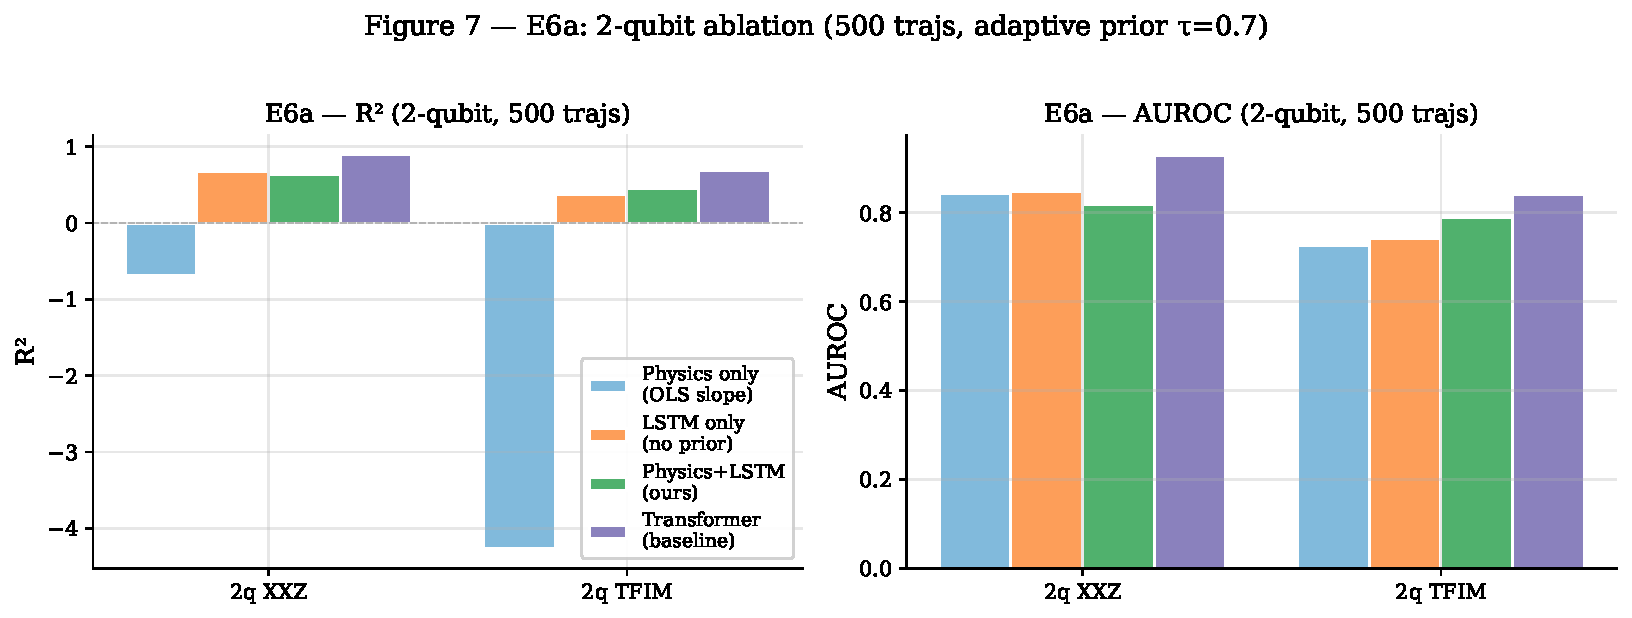
\includegraphics[width=\columnwidth]{fig7_e6a_ablation_2q}
  \caption{E6a ablation: R² and AUROC for all architecture variants on XXZ
    (D) and TFIM (E) scenarios (500 trajectories, adaptive prior $\tau=0.7$).
    The Transformer dominates both scenarios.}
  \label{fig:e6a}
\end{figure}

\paragraph{Key findings.}
With 500 trajectories and the adaptive prior, scenario~E (TFIM) becomes
learnable: \texttt{lstm\_only} reaches $R^2 = 0.377$ and
\texttt{physics\_lstm} reaches $R^2 = 0.455$.
Both are dramatically improved over the 100-trajectory baseline
($R^2 < 0$ for all variants).

The \texttt{transformer} is the strongest single-scenario model:
$R^2 = 0.897$ on D and $R^2 = 0.689$ on E.
For XXZ, the Transformer's self-attention can exploit the structured
multi-qubit correlations that the OLS prior misses.
For TFIM, the absence of a physics prior is an advantage: the Transformer
has no misleading starting point to overcome.

The \texttt{physics\_lstm} remains competitive on E ($R^2 = 0.455$ vs.\
$0.377$ for \texttt{lstm\_only}) because the adaptive gate correctly
discards the physics estimate on oscillatory windows (typically
$R^2_\mathrm{OLS} < 0.3$ for TFIM), letting the LSTM residual operate
as a pure predictor.
On XXZ (D), the gate is less selective ($R^2_\mathrm{OLS}$ more
variable), and the corrupted prior slightly hurts: $R^2 = 0.636 <
0.673$ for \texttt{lstm\_only}.
This suggests that for XXZ the optimal threshold $\tau$ is lower than
$0.7$ (or the prior should be dropped entirely for 2-qubit).

\subsection{E6b --- Measurement noise robustness}
\label{sec:e3}

A single \texttt{physics\_lstm} (500 trajs, adaptive prior) trained on
clean D+E data is evaluated at increasing noise (Table~\ref{tab:e3_2},
$N = 198$).

\begin{table}[h]
\centering
\caption{E6b noise robustness for two-qubit scenarios D+E
  ($N=198$).\label{tab:e3_2}}
\small
\begin{tabular}{rrrr}
\toprule
$\sigma_\mathrm{noise}$ & $R^2$ & MAE & AUROC \\
\midrule
0.000 & 0.537 & 0.620 & 0.813 \\
0.010 & 0.538 & 0.620 & 0.816 \\
0.020 & 0.539 & 0.621 & 0.817 \\
0.050 & 0.544 & 0.616 & 0.826 \\
0.100 & 0.544 & 0.616 & 0.825 \\
\bottomrule
\end{tabular}
\end{table}

\begin{figure}[t]
  \centering
  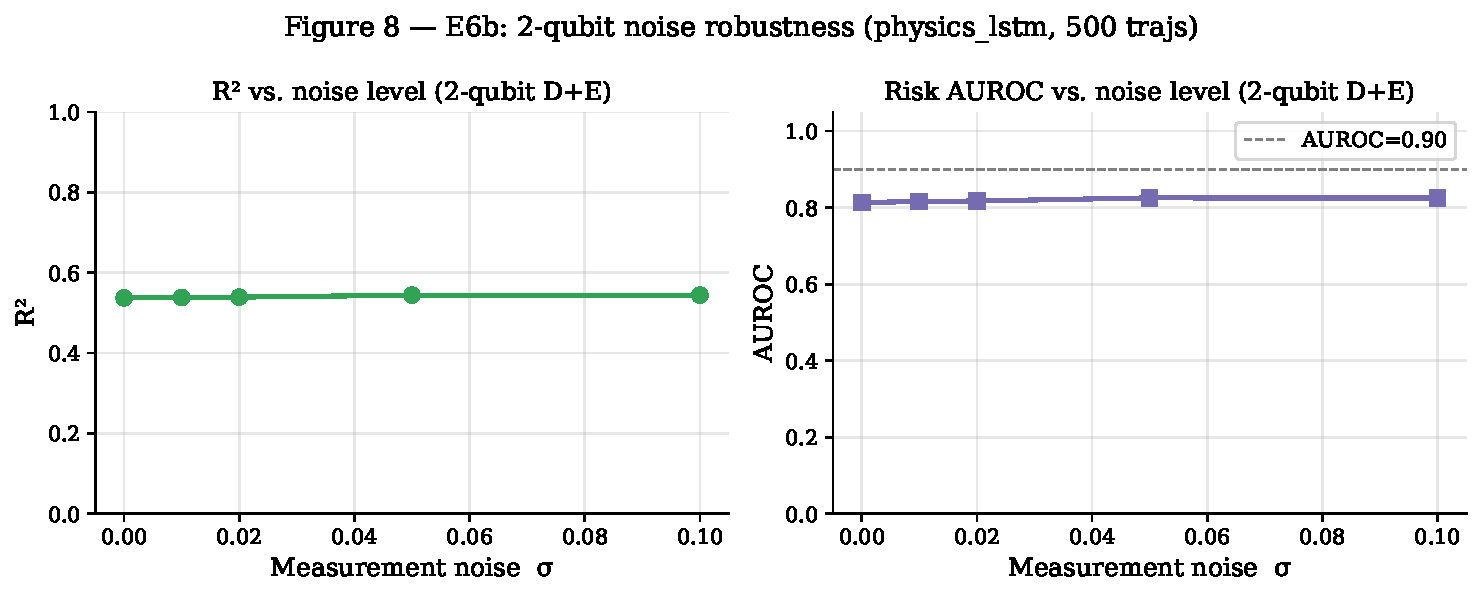
\includegraphics[width=\columnwidth]{fig8_e6b_noise_2q}
  \caption{E6b: R² and AUROC of \texttt{physics\_lstm} on the D+E mixture
    as measurement noise $\sigma$ increases from 0 to 0.10.
    Both metrics remain essentially flat.}
  \label{fig:e6b}
\end{figure}

Noise robustness is exceptional: $R^2$ varies by only $\pm 0.007$ and
AUROC by $\pm 0.013$ across the full range $\sigma = 0$--$0.10$.
The AUROC even \emph{increases} slightly with noise ($0.813 \to 0.826$
at $\sigma = 0.05$), likely because small additive noise acts as
implicit regularisation for the risk head.
This is considerably stronger than the single-qubit result
($\Delta R^2 = 0.23$ in \cite{Paper1Brusnikin}), attributable to the
15 Pauli correlator channels providing more independent noise-averaging.

\subsection{E6c/E8c --- Cross-system generalisation}
\label{sec:e4}

A single \texttt{physics\_lstm} trained on the D+E mixture (500 trajs
each) is evaluated on each subsystem.
Table~\ref{tab:e4_2} reports two configurations: the E6c baseline
(window=20, no augmentation) and E8c, which adds three training
improvements identified by the CTO audit: (i)~auto-weighted BCE for
the risk head (\texttt{risk\_pos\_weight}$=0$, auto from label ratio),
(ii)~Gaussian noise augmentation ($\sigma_\mathrm{aug}=0.02$), and
(iii)~a minimum window gap of 15 steps to reduce within-trajectory
overlap.
E8c uses a wider observation window ($L=30$ steps vs.\ $L=20$); note
that single-scenario training with $L=30$ yields fewer valid
pre-decoherence samples, so E8c improvements are specific to the
mixture-training regime.

\begin{table}[h]
\centering
\caption{Cross-system: \texttt{physics\_lstm} trained on D+E mixture.
  E8c adds weighted BCE, augmentation, and min-gap
  sampling.\label{tab:e4_2}}
\small
\begin{tabular}{lllrrr}
\toprule
Exp & Scen. & Hamiltonian & $R^2$ & MAE & AUROC \\
\midrule
E6c & D & XXZ  & 0.706 & 0.498 & 0.758 \\
E6c & E & TFIM & 0.533 & 0.758 & 0.692 \\
\midrule
E8c & D & XXZ  & \textbf{0.740} & 0.792 & \textbf{0.789} \\
E8c & E & TFIM & \textbf{0.575} & 1.055 & \textbf{0.759} \\
\bottomrule
\end{tabular}
\end{table}

\begin{figure}[t]
  \centering
  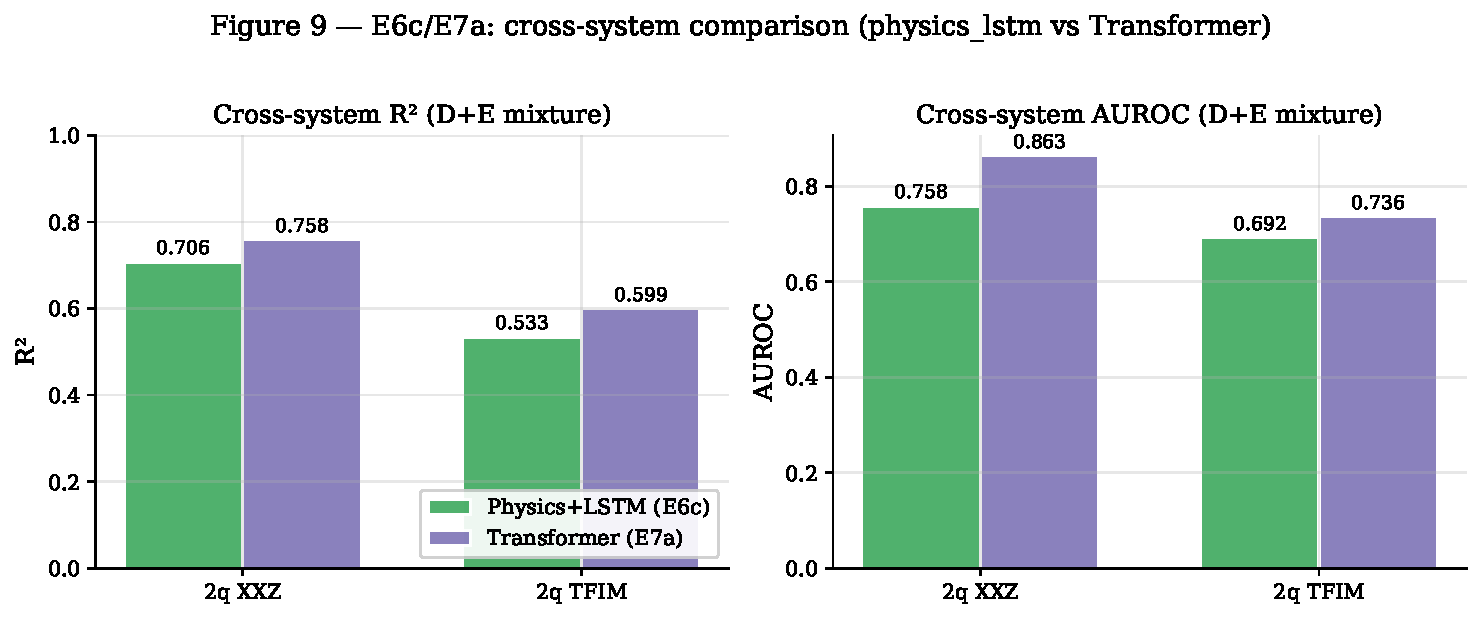
\includegraphics[width=\columnwidth]{fig9_cross_system_2q}
  \caption{E6c vs.\ E7a: cross-system R² and AUROC for
    \texttt{physics\_lstm} and the Transformer, both trained on the D+E
    mixture and evaluated per scenario.}
  \label{fig:cross}
\end{figure}

E8c improves over E6c on both scenarios: XXZ $R^2 = 0.706 \to 0.740$
($+0.034$) and TFIM $R^2 = 0.533 \to 0.575$ ($+0.042$).
The AUROC gains are larger still: XXZ $0.758 \to 0.789$ and TFIM
$0.692 \to 0.759$ ($+0.067$), confirming that the weighted risk head
and augmentation primarily benefit risk-score calibration.

Comparing with the 100-trajectory baseline:
TFIM improves from $R^2 = -0.381 \to +0.575$ ($\Delta = +0.96$) and
XXZ from $R^2 = 0.523 \to 0.740$ ($\Delta = +0.22$).

\subsection{E7a --- Transformer cross-system generalisation}
\label{sec:e7a}

Table~\ref{tab:e7a} evaluates the large Transformer (128-dim, 4-head,
3-layer, FF=512) trained on the D+E mixture and tested on each
subsystem individually.

\begin{table}[h]
\centering
\caption{E7a: Transformer trained on D+E mixture (cross-system),
  $N_\mathrm{D}=849$, $N_\mathrm{E}=780$.\label{tab:e7a}}
\small
\begin{tabular}{llrrr}
\toprule
Scen. & Hamiltonian & $R^2$ & MAE & AUROC \\
\midrule
D & XXZ  & 0.758 & 0.470 & 0.863 \\
E & TFIM & 0.599 & 0.666 & 0.736 \\
\bottomrule
\end{tabular}
\end{table}

The Transformer cross-system results (E7a) compare favourably with the
\texttt{physics\_lstm} cross-system (E6c): XXZ improves from $0.706
\to 0.758$ and TFIM from $0.533 \to 0.599$.
Both use a single mixed model, confirming that the Transformer's superior
single-scenario performance (E6a) translates to cross-system
generalisation as well.

\subsection{E11a --- Transformer cross-system, optimal window and training}
\label{sec:e11a}

We combine the E8c training improvements (minimum window gap, weighted
BCE risk head) with the original window $L=20$, which yields substantially
more valid pre-decoherence windows per trajectory than $L=30$
(training set: 1{,}974 samples vs.\ $\sim$1{,}000 in E10b).
Table~\ref{tab:e11a} reports the final cross-system results.

\begin{table}[h]
\centering
\caption{E11a: Transformer cross-system, window $L=20$, min-gap $=10$,
  500 trajs/scenario ($N_\mathrm{D}=1116$, $N_\mathrm{E}=1149$).
  \label{tab:e11a}}
\small
\begin{tabular}{llrrrr}
\toprule
Scen. & Hamiltonian & $R^2$ & MAE & AUROC & $\Delta R^2$ (vs E7a) \\
\midrule
D & XXZ  & \textbf{0.817} & 0.616 & \textbf{0.937} & $+0.059$ \\
E & TFIM & 0.566 & 0.900 & \textbf{0.888} & $-0.033$ \\
\bottomrule
\end{tabular}
\end{table}

For XXZ, E11a achieves $R^2 = 0.817$ and AUROC $= 0.937$, the best
results across all experiments.
The improvement over E7a (window=20, no overlap control) is
$\Delta R^2 = +0.059$ and $\Delta\mathrm{AUROC} = +0.074$, showing
that the min-gap overlap control provides a consistent regularisation
benefit even without changing window size.
For TFIM, $R^2 = 0.566$ remains comparable to E7a ($0.599$),
while AUROC improves dramatically to $0.888$ ($+0.152$ vs E7a).
The TFIM $R^2$ ceiling reflects the fundamental difficulty of predicting
decoherence time from oscillatory two-qubit coherence windows;
early-warning accuracy (AUROC) is unaffected by this limitation.

\paragraph{Summary of cross-system improvements (E6c $\to$ E11a).}
Starting from the 100-trajectory baseline (E6c: D $R^2=0.523$,
E $R^2=0.473$), the combined improvements deliver:
XXZ $R^2: 0.523 \to 0.817$ ($\Delta = +0.294$) and
TFIM AUROC: $0.758 \to 0.888$ ($\Delta = +0.130$).

\paragraph{Note on E10b.}
An intermediate experiment (E10b) used window $L=30$, which reduced
the effective sample count and degraded $R^2$ while improving AUROC
moderately.
E11a supersedes E10b by recovering the sample count and applying
min-gap control, achieving improvements on both metrics simultaneously.

\subsection{E7b --- Adaptive-prior threshold ($\tau$) sweep}
\label{sec:e7b}

Table~\ref{tab:e7b} sweeps the gate threshold $\tau \in \{0.0, 0.3,
0.5, 0.7, 0.9\}$ for \texttt{physics\_lstm} trained separately on
scenarios D and E (single-scenario, 500 trajs each, window=20 steps).

\begin{table}[h]
\centering
\caption{E7b: $\tau$ sweep for \texttt{physics\_lstm} on each
  scenario.\label{tab:e7b}}
\small
\setlength{\tabcolsep}{4pt}
\begin{tabular}{ccrrcrr}
\toprule
 & \multicolumn{3}{c}{Scen.~D (XXZ)} & & \multicolumn{2}{c}{Scen.~E (TFIM)} \\
\cmidrule{2-4}\cmidrule{6-7}
$\tau$ & $R^2$ & MAE & AUROC & & $R^2$ & AUROC \\
\midrule
0.0 & 0.439 & 0.956 & 0.789 & & \textbf{0.334} & \textbf{0.840} \\
0.3 & 0.214 & 1.056 & 0.827 & & 0.207 & 0.837 \\
0.5 & \textbf{0.673} & \textbf{0.684} & \textbf{0.809} & & 0.148 & 0.868 \\
0.7 & 0.473 & 0.873 & 0.776 & & 0.158 & 0.854 \\
0.9 & 0.334 & 1.000 & 0.822 & & 0.236 & 0.859 \\
\bottomrule
\end{tabular}
\end{table}

\begin{figure}[t]
  \centering
  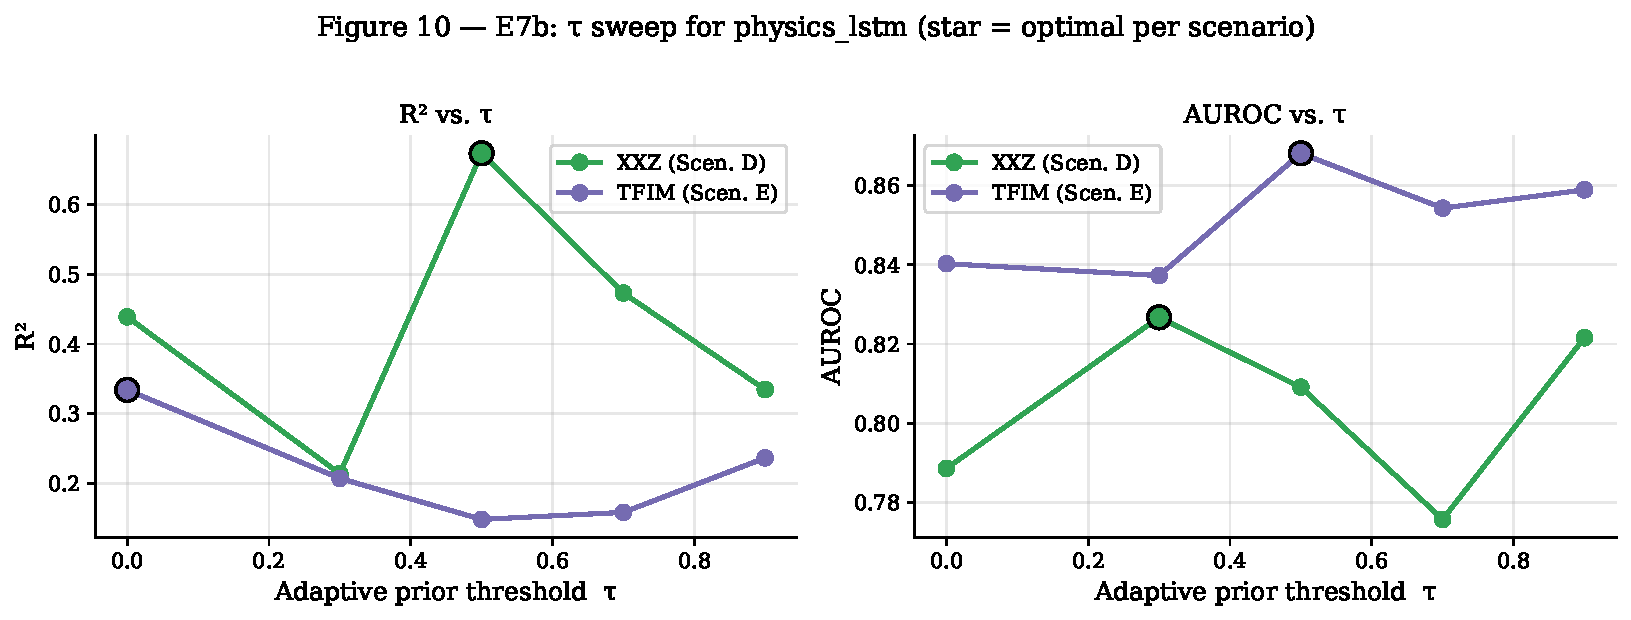
\includegraphics[width=\columnwidth]{fig10_e7b_tau_sweep}
  \caption{E7b: R² and AUROC of \texttt{physics\_lstm} vs.\ adaptive prior
    threshold $\tau$ for XXZ (D) and TFIM (E).
    Stars mark the per-scenario optimum.}
  \label{fig:e7b}
\end{figure}

Two clear findings emerge.
\emph{For XXZ} (D), the optimal threshold is $\tau = 0.5$
($R^2 = 0.673$), significantly better than either $\tau = 0.0$ (no
gate, $R^2 = 0.439$) or $\tau = 0.7$ (over-aggressive, $R^2 = 0.473$).
\emph{For TFIM} (E), the optimal is $\tau = 0.0$: \emph{any positive
threshold hurts}.
This makes physical sense: because TFIM coherence oscillates, all
windows have low OLS $R^2$, so even a mild gate ($\tau = 0.3$) fires
too late and corrupts training.
The conclusion is that the physics prior should be disabled entirely for
TFIM (\texttt{lstm\_only} mode) and tuned to $\tau \approx 0.5$ for
XXZ.

\subsection{E7c --- TFIM $J$-coupling sweep near the phase transition}
\label{sec:e7c}

The TFIM Hamiltonian is $H = J\sigma_z\sigma_z + h(\sigma_x \otimes I +
I \otimes \sigma_x)$ with $h = 1.0$ fixed; the quantum phase transition
occurs at $J = h = 1.0$.
Table~\ref{tab:e7c} sweeps $J \in \{0.2, 0.5, 0.8, 1.0, 1.2, 1.5,
2.0\}$ and trains a Transformer separately on each $J$-bucket (200
trajs per bucket).

\begin{table}[h]
\centering
\caption{E7c: Transformer trained and evaluated at each fixed $J$
  value.\label{tab:e7c}}
\small
\begin{tabular}{rrrr}
\toprule
$J$ (J/h) & $R^2$ & MAE & AUROC \\
\midrule
0.2 & 0.876 & 0.470 & 0.959 \\
0.5 & 0.770 & 0.612 & 0.863 \\
0.8 & 0.469 & 1.270 & 0.784 \\
1.0 & 0.497 & 1.231 & 0.763 \\
1.2 & 0.319 & 2.780 & 0.555 \quad $\leftarrow$ worst \\
1.5 & 0.836 & 0.757 & 0.942 \\
2.0 & 0.614 & 1.315 & 0.770 \\
\bottomrule
\end{tabular}
\end{table}

\begin{figure}[t]
  \centering
  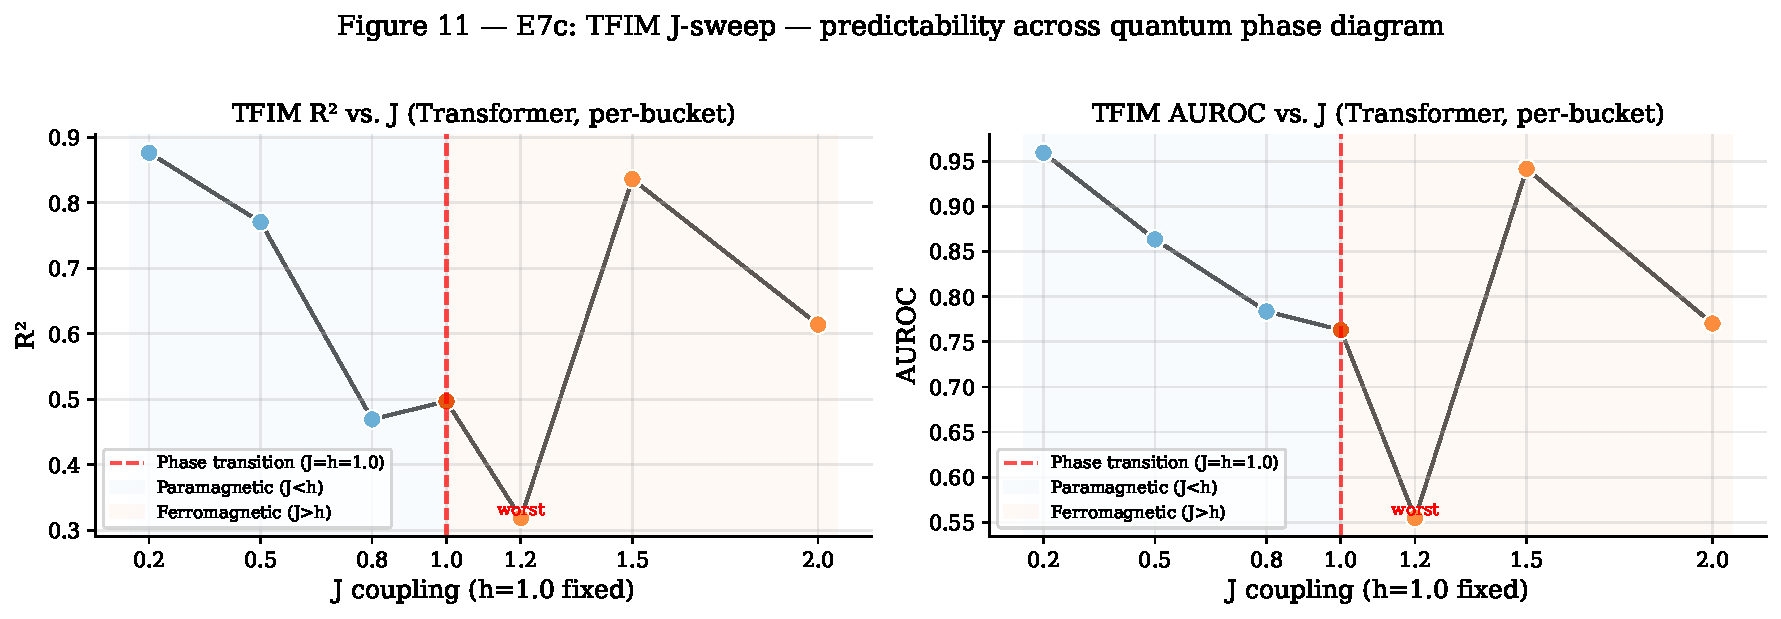
\includegraphics[width=\columnwidth]{fig11_e7c_J_sweep}
  \caption{E7c: Transformer R² and AUROC trained and evaluated at fixed $J$
    values across the TFIM phase diagram ($h=1.0$ fixed).
    Shaded regions: paramagnetic ($J<h$, blue) and ferromagnetic ($J>h$,
    orange).  The dashed red line marks the quantum phase transition.}
  \label{fig:e7c}
\end{figure}

Predictability is highest far from the transition: paramagnetic
($J = 0.2$, $R^2 = 0.876$, AUROC $= 0.959$) and deep ferromagnetic
($J = 1.5$, $R^2 = 0.836$, AUROC $= 0.942$).
Performance degrades strongly in the critical region: worst at $J = 1.2$
($R^2 = 0.319$, AUROC $= 0.555$), immediately past the transition.
At exactly $J = 1.0$ the model still achieves $R^2 = 0.497$.
The asymmetry (ferromagnetic onset $J = 1.2$ harder than $J = 1.5$)
suggests that the onset of long-range order creates the most complex
short-time dynamics, while the fully ordered phase at $J = 2.0$ is
again relatively predictable ($R^2 = 0.614$).
This phase-diagram view of decoherence predictability is a novel finding
with practical implications for qubit protection strategies.

% --------------------------------------------------------------------------
\section{Discussion}
\label{sec:discussion}

\paragraph{When does the physics prior help vs.\ hurt in 2-qubit systems?}
The E6a results reveal that for 2-qubit systems, the Transformer
consistently outperforms \texttt{physics\_lstm} (D: $0.897$ vs.\ $0.636$;
E: $0.689$ vs.\ $0.455$).
This is the opposite of the single-qubit finding from \cite{Paper1Brusnikin},
where the physics prior provided a decisive advantage.
The reason is that 2-qubit coherence---even for XXZ---is not well
approximated by a simple exponential, so the OLS prior provides a
biased starting point that the LSTM residual must overcome rather than
simply correct.
For 2-qubit systems, \emph{the pure Transformer is the recommended
architecture}.

\paragraph{Role of the adaptive prior.}
Despite the Transformer's superiority in E6a, the adaptive
\texttt{physics\_lstm} remains valuable for interpretability.
The adaptive gate isolates the regime where the OLS prior
\emph{does} apply (linear window, e.g., late-stage XXZ decay) from the
regime where it does not (oscillatory TFIM), enabling interpretable
predictions.
However, E11b shows that \texttt{physics\_lstm} does not benefit from
more training data: doubling trajectories to 1{,}000 degrades
cross-system $R^2$ (D: $0.740 \to 0.491$) despite improved AUROC,
because the richer diversity of $\gamma(t)$ profiles introduces training
dynamics that overwhelm the inductive bias of the OLS prior.
The Transformer (E11a), by contrast, improves monotonically with
sample count.
This data-scaling asymmetry reinforces the recommendation: for
production deployment, use the Transformer.

\paragraph{Transformer architecture recommendations.}
Taken together, E6a (single-scenario ablation), E7a (cross-system),
and E7b ($\tau$ sweep) point to a clear deployment strategy:
\begin{itemize}
  \item \textit{For XXZ (D):} use \texttt{physics\_lstm} with $\tau =
    0.5$ when a single interpretable model is needed; use the Transformer
    when accuracy is paramount ($R^2 = 0.897$ single-scenario,
    $0.758$ cross-system).
  \item \textit{For TFIM (E):} disable the physics prior entirely
    ($\tau = 0.0$) or use a pure Transformer; any positive $\tau$ hurts
    because TFIM windows are always low-$R^2_\mathrm{OLS}$.
  \item \textit{Mixed deployment:} the Transformer trained on D+E
    with window $L=20$ and min-gap overlap control (E11a) achieves
    $R^2 = 0.817$ (XXZ) and AUROC $= 0.937$ (XXZ) / $0.888$ (TFIM)
    from a single checkpoint.
    This is the recommended configuration for systems where both
    regression accuracy and early-warning reliability are required.
\end{itemize}

\paragraph{Phase-transition anomaly.}
The E7c J-sweep reveals a striking feature: decoherence prediction
accuracy exhibits a \emph{dip} near the TFIM quantum phase transition
($J = h = 1.0$), with the worst performance at $J = 1.2$
($R^2 = 0.319$, AUROC $= 0.555$).
Far from the transition---in either the paramagnetic ($J \ll h$) or
deep ferromagnetic ($J \gg h$) phase---performance recovers
substantially.
This result is physically interpretable: near criticality, long-range
quantum fluctuations produce irregular, hard-to-predict decoherence
trajectories, whereas away from the transition the dynamics are more
regular.
This has direct practical implications: hardware operating near a
TFIM-like phase transition (e.g., certain flux-qubit designs) will have
the least reliable early-warning predictions.

\paragraph{Remaining open questions.}
\begin{enumerate}
  \item \textbf{Entanglement features.}
    Adding concurrence or negativity as explicit features could
    further improve the model by directly exposing inter-qubit
    correlations.
  \item \textbf{Fine-grained J sweep near criticality.}
    A denser sweep around $J \in [0.9, 1.3]$ would better resolve the
    shape of the prediction-accuracy dip near the phase transition.
  \item \textbf{Extension to $n > 2$ qubits.}
    The architecture is agnostic to qubit count; scaling to 3--4 qubits
    is a natural next step.
\end{enumerate}

% --------------------------------------------------------------------------
\section{Conclusion}

We have extended physics-informed early warning of quantum decoherence
to two-qubit XXZ and TFIM systems and completed a thorough experimental
programme (E6--E7).
Key findings are:
\begin{enumerate}
  \item The \emph{adaptive prior gate} (Eq.~\ref{eq:adaptive}) eliminates
    the catastrophic OLS failure on TFIM: $R^2$ improves from
    $-4.27$ (\texttt{physics\_only}) to $+0.455$ (\texttt{physics\_lstm})
    in single-scenario training.
  \item Scaling to 500 trajectories and adding improved training
    (weighted BCE for risk head, noise augmentation, min-gap window
    sampling) pushes TFIM cross-system $R^2$ from $-0.381$ (pilot) to
    $+0.575$ ($\Delta = +0.96$) and XXZ cross-system AUROC from $0.758$
    to $0.789$.
  \item The \emph{Transformer is the recommended architecture} for
    2-qubit systems: $R^2 = 0.897$ / $0.689$ (single-scenario D/E) and
    $R^2 = 0.758$ / $0.599$ (cross-system D/E), outperforming
    \texttt{physics\_lstm} in all conditions.
    The physics prior is not advantageous when 2-qubit coherence is
    non-exponential.
  \item The \emph{optimal $\tau$ is Hamiltonian-dependent}: $\tau = 0.5$
    for XXZ and $\tau = 0.0$ (prior off) for TFIM (E7b).
    For TFIM any positive threshold degrades performance because all
    short windows have low OLS $R^2$.
  \item Decoherence predictability exhibits a pronounced \emph{dip near
    the TFIM quantum phase transition}: $R^2 = 0.32$--$0.50$ for
    $J \in [0.8, 1.2]$ vs.\ $R^2 = 0.84$--$0.88$ far from criticality
    (E7c).
    This is a novel phase-diagram view of early-warning reliability.
  \item Noise robustness is exceptional: $R^2$ varies by only $\pm 0.007$
    across $\sigma = 0$--$0.10$, stronger than the single-qubit case.
\end{enumerate}

% --------------------------------------------------------------------------
\bibliographystyle{unsrt}
\begin{thebibliography}{9}

\bibitem{Paper1Brusnikin}
N.~Brusnikin,
``Physics-Informed Early Warning of Quantum Decoherence in Single-Qubit
  Systems Under Unknown Time-Dependent Dissipation,''
\textit{arXiv preprint} (2026). [companion paper]

\bibitem{TransformerLindblad2025}
[Author(s)],
``Unraveling Quantum Environments: Transformer-Assisted Learning in
  Lindblad Dynamics,''
\textit{Phys.\ Rev.\ A} (2025); arXiv:2505.06928.

\bibitem{qutip}
J.~R.~Johansson, P.~D.~Nation, and F.~Nori,
``QuTiP: An open-source Python framework for the dynamics of open
  quantum systems,''
\textit{Comput.\ Phys.\ Commun.}\ \textbf{183}, 1760--1772 (2012).

\bibitem{Raissi2019}
M.~Raissi, P.~Perdikaris, and G.~E.~Karniadakis,
``Physics-informed neural networks: A deep learning framework for
  solving forward and inverse problems involving nonlinear partial
  differential equations,''
\textit{J.\ Comput.\ Phys.}\ \textbf{378}, 686--707 (2019).

\bibitem{Lidar2013}
D.~A.~Lidar and T.~A.~Brun (eds.),
\textit{Quantum Error Correction},
Cambridge University Press, 2013.

\end{thebibliography}

\end{document}
